\documentclass[11pt]{article}
\usepackage[margin=0.8in]{geometry}

\usepackage[comma]{natbib}
\usepackage{color}
\usepackage{mdwlist}
\usepackage{graphicx}
\usepackage{url}
\usepackage{comment}

% a bit more spacing between paragraphs
\setlength{\parskip}{1ex plus 0.5ex minus 0.5ex}

% epigraphs, used after section heads
%\usepackage{epigraph}
% set width for \epigraph{}{}
%\setlength{\epigraphwidth}{.8\textwidth}
\newcommand*{\epigraph}[2]{{\renewcommand{\baselinestretch}{1}\normalfont\emph{#1}\hfill---#2\par\vspace{1ex}}}

\newcommand{\TODO}[1]{\begin{quotation}\noindent\color{blue}\textbf{ToDo}: #1\end{quotation}}

%  Abbreviations for cross-references
\newcommand*{\figref}[1]{Figure~\ref{#1}}
\newcommand*{\tabref}[1]{Table~\ref{#1}}
\newcommand*{\secref}[1]{Section~\ref{#1}}
\newcommand*{\eqref}[1]{Eqn.~(\ref{#1})}

% abbreviations
\newcommand{\Cent}[1]{#1$^{th}$ century}
%\newcommand{\keywords}[1]{\par\noindent\textbf{Key words:} #1}
\newcommand*{\boldital}[1]{\textit{\textbf{#1}}}
\newcommand*{\degree}[1]{\ensuremath{{#1}^{\circ}}}

\newcommand*{\scat}{scatterplot}
\newcommand*{\scats}{scatterplots}
\newcommand*{\scatmat}{scatterplot matrix}
\newcommand*{\scatmats}{scatterplot matrices}

%\bibliographystyle{abbrvnat-last}
\bibliographystyle{abbrvnat-apa-nourl}
\providecommand{\Loc}[1]{\textsf{#1}}

\begin{document}

\title{The Milestones Project: \\ A Database for the History of Data Visualization}
\author{Michael Friendly%
\thanks{This work was supported by Grant OGP0138748 from the National Sciences and Engineering Research Council of Canada to Michael Friendly.
  We are grateful to Dan Denis, Stephen Stigler, Ben Shneiderman ... for constructive comments on this chapter.
  }
 \and Matthew Sigal 
 \and Derek Harnanansingh}
\date{\today}

\maketitle

\begin{abstract}
%\TODO{Revise, incorporating some/all of Matt's changes, presently just comments in the .tex file; in general, abstract %should be shortened.}
\begin{comment}
Re-reading the abstract, I think it could be rephrased slightly to update the language with more modern historical scholarship (most of the changes are in paragraph 1).  Here is what I propose:

Methods of data visualization have evolved substantially over their relatively brief history.
Landmarks in this story were the first thematic maps in the 1600s, the invention of the bar chart and the line graph in the early 1800s,
and the dynamic and interactive graphics of today.  While these developments have been previously detailed in various micro-histories,
they were aimed at a privileged and academic audience, and a publicly accessible and free space to house a macro-history in its totality did not exist.

The purpose of this chapter is threefold:
first, to introduce the reader our solution to this absence through an online resource called the Milestones Project.
This website highlights important events in the history of data visualization, and enables users to interactively travel through time to see and explore the
context that surrounded their developments.
Secondly, we present some striking visual examples that deal with conveying aspects of history over time, drawn from this resource.
Finally, the Milestones database itself will be used to showcase how such a resource can serve as ``data'' for \emph{statistical historiography},
which entails the use of statistical and graphical methods for the analysis and understanding of historical innovations, developments, and trends.
\end{comment}

Methods of data visualization have evolved substantially over their history.
Some landmarks in this story were the first thematic maps in the 1600s, the invention of the bar chart and line graph in the early 1800s,
and the dynamic and interactive graphics of today.  
While these developments have been previously detailed in various written micro-histories, 
there has never been an attempt to collect a complete, macro-history in a single place for study, search or query, and even data analysis or graphics based on this history.

\begin{comment}
Approaches to modern data visualization have evolved substantially from the first thematic maps of the 1600s and the first bar charts and line graphs in the early 1800s to the dynamic and interactive graphics of today. Over the course of this history, there have been many detailed written studies, both comprehensive and on particular aspects. But there has never been an attempt to collect this history in a single place for display, search or query and even data analysis or graphics based on this history.
\end{comment}

The purpose of this chapter is threefold: first, to introduce the reader to our solution: an online resource called the Milestones Project. This web site details  important events in the history of data visualization, and enables users to interactively travel through time to see and explore the context that surrounded their developments. 
Secondly, we present some striking visual examples that deal with conveying aspects of history over time, drawn from this resource.

Finally, the Milestones database will be used to showcase how such a resource can serve as ``data'' for \emph{statistical historiography}, which entails the use of statistical and graphical methods for the analysis and understanding of historical innovations, developments, and trends.
\end{abstract}

\section{Introduction}\label{sec:intro}
\epigraph{If you would understand anything, observe its beginning and its development.}{Aristotle}

Questions regarding the history of data visualization are (or at least should be) of great importance to historians of science, to current developers of graphical methods for statistical analysis and the related info-vis community, as well those just interested in the history of ideas. In the history of science, diagrams, graphs, maps and other visualizations have often played important roles in discoveries that arguably might not have been achieved otherwise.%
\footnote{
	Some salient examples are:
	Francis Galton's 1861 discovery of anti-cyclonic movement of wind around low-pressure areas from contour maps; Edward Maunder's ``butterfly diagram'' of the variation of sunspots over time leading to the	discovery of the ``Maunder minimum,'' from 1645--1715; and Henry Moselely's 1913 discovery of the concept of atomic number, based largely on graphical analysis (a plot of serial numbers of the elements vs. square root of frequencies from their X-ray spectra).
}
At the same time, in the fields of statistical graphics and information visualization, developers often create ``new'' methods without any appreciation that they have deep roots in the past.%
\footnote{
  For example, mosaic displays for frequency tables were thought to have been invented by \citet{HartiganKleiner:81} and extended to show the pattern of residuals in loglinear models by \citet{Friendly:94a}. But it turns out that the essential idea behind this area-based display is goes back to Georg von Mayr in 1877 \citep{Friendly:2002:mosahist}.
}

These two perspectives provided the motivation for the development of the Milestones Project. 
\begin{comment}
Rephrase the second sentence: Previous historical accounts of events, ideas and techniques that relate \emph{inter alia} to modern data visualizations were fragmented - scattered across a wide number of fields, publications, and languages (insert footnote here).  The present project's goal was to bring these resources together into a publicly and freely available database.
\end{comment}
This stemmed from the fact that historical accounts of events, ideas and techniques that relate \emph{inter alia} to modern data visualization were fragmented and scattered across a wide number of fields.%
\footnote{
Among these are general histories in the fields of probability \citep{Hald:1990}, statistics \citep{Pearson:1978,Porter:1986,Stigler:1986}, astronomy \citep{Riddell:1980}, cartography \citep{WallisRobinson:87}. More specialized accounts focus on the early history of graphic recording \citep{HoffGeddes:1959,HoffGeddes:1962}, statistical graphs \citep{Funkhouser:1936,Funkhouser:1937,Royston:1970,Tilling:1975}, fitting equations to empirical data \citep{Farebrother:1999}, cartography \citep{Friis:1974,Kruskal:1977}, thematic mapping \citep{FriendlyPalsky:2007,Palsky:1996,Robinson:1982}, and so forth.
}

When this work began in the mid-1990s, there were no accounts or resources that spanned the entire development of visual thinking and the visual representation of data across different disciplines and perspectives. The Milestones Project began simply as an attempt to collate these diverse contributions into a single, comprehensive listing, organized chronologically, that contained representative images, references to original sources, and links to further discussion -- a source for ``One-Stop Shopping'' on the history of data visualization.

In \secref{sec:project}, we describe the evolution and structure of the Milestones Project. \secref{sec:vistime} presents some historical and modern approaches to one self-referential question: how can data visualization be applied to its own history? \secref{sec:historiography} introduces another self-referential topic we call \emph{statistical historiography}, which entails the use of statistical and graphical methods for the analysis and understanding of historical innovations, developments, and trends. But first we give some brief vignettes of historical topics and questions for which the Milestones Project has proved invaluable in our own research.

\begin{comment}
\begin{itemize*}
 \item The first statistical graph?
 \item Who invented the scatterplot?
 \item The origin of mosaic displays
 \item The Golden Age of statistical graphics
\end{itemize*}
\end{comment}

\subsection{The first statistical graph}
In the history of statistical graphics \citep{Friendly:06:hbook}, as in other artful sciences, there are a number of inventions and developments that can be considered ``firsts'' in these fields. The catalog of the Milestones Project \citep{FriendlyDenis:01} lists 70 events that can be considered to be the initial use or statement of an idea, method or technique that is now commonplace, but there is probably no question more fundamental than that of the first visual representation of statistical data.

In \citet{Friendly-etal:2010:langren} we argue that the 1-dimensional line graph shown in \figref{fig:langren-google-overlay} by Michael Florent van Langen \citep{Langren:1644} should be accorded this honour. The graph shows 12 estimates of the distance in longitude between Toledo and Rome, overlaid on a modern map. van Langren used this to demonstrate that these estimates were all subject to large errors and to
propose to King Phillip of Spain that only he had a sufficiently precise method for the determination of longitude for navigation at sea.

\begin{comment}
I've updated this image to make it clearer.  I didn't like how the original text got lost among the Google Maps text before.
\end{comment}

\begin{figure}[htb]
 \centering
 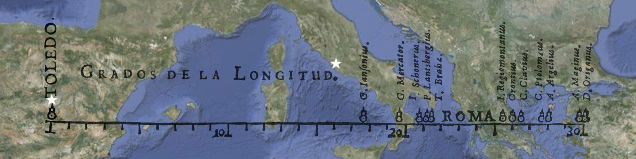
\includegraphics[width=\textwidth]{fig/langren-google-overlay2}
 \caption{van Langren's 1644 graph, re-scaled and overlaid on a modern map of Europe. Toledo is located at lat/long %39$^o$51$^'$36$^\"$N, 4$^o$01$^'$48$^\"$W
(\degree{+39.86}N, \degree{-4.03}W), Rome is located at (\degree{+41.89}N, \degree{+12.5}W), both shown by markers on the map.  This image makes clear what van Langren wished to communicate: the wide variability of the estimates, but also shows how far the estimates were biased.}%
\label{fig:langren-google-overlay}
\end{figure}

The telling of van Langren's story not only turned out to involve astronomy, archival research, details of patronage in the \Cent{17}, and even an unsolved problem of cryptography, but also serves as an example of statistical historiography.  The Milestones Project provided the infrastructure for this research -- through the use of a time-based, cross-referenced catalog of images, references and links to related work, van Langren's tale was able to be studied and reported upon.

\subsection{Who invented the scatterplot?}
Although there are earlier precursors, the main graphical methods used today --
pie charts, line graphs and bar charts -- are generally attributed to William Playfair around the beginning of the \Cent{19} \citep{Playfair:1786,Playfair:1801}. Each of these are essentially univariate displays, showcasing some aspect of a single variable. 

A logical next step would be to discover a method that could reveal the relationship between two variables, which we now know as the scatterplot.  By \citeyear{Galton:1886}, Francis Galton had utilized this truly bivariate display in his discovery of correlation and regression, and it would become an essential tool for the presentation of multivariate statistics. However, he may not have been the first to use this graphical technique, and it is surprising that no one is widely credited with its invention.

In \citet{FriendlyDenis:05:scat}, we delved into this mystery.  This involved tracing the early origins of ideas related to the scatterplot, which led to two compelling narratives: how, in Playfair's time, it was nearly impossible to think about and visualize bivariate relationships; and, later, how the scatterplot was quintessential for Galton's visual insights that would lead to the rise of modern statistics and graphics. It was the resources available in the Milestones Project that allowed us to focus upon the events between these two extremities and attribute the essential ideas of the scatterplot to J. F. W. Herschel in two 1832 papers.

\subsection{The Golden Age of statistical graphics}

In our initial web presentation of the Milestones Project, it proved convenient
to sub-divide the history of data visualization into epochs, each of which turned
out to be describable by coherent themes.  For reasons we describe later, one
period turned out to be particularly noteworthy, both for the sheer number of
contributions, and for the beauty and elegance of their execution. We call this period, from roughly 1850 to 1900 ($\pm 10$), the Golden Age of statistical graphics \citep{Friendly:2008:golden}.

\figref{fig:mileyears4} shows the time distribution of the 260 significant events that had been included in the Milestones Project database by 2007, demarcated by the labels we used for epochs. In \citet{Friendly:2008:golden}, we traced the origin of this period in terms of the infrastructure required to produce such an explosive growth of contributions to data visualization, and found three primary sources: the systematic data collection by state agencies, the rise in popularity of statistical and visual thinking, and the enabling developments of technological innovations.
%% one figure
\begin{figure}[!htb]
  \centering
  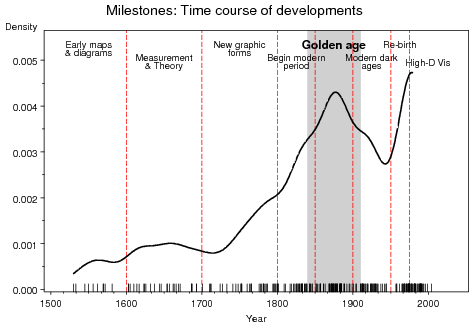
\includegraphics[width=.9\textwidth,clip]{fig/mileyears4}
  \caption{The time distribution of events considered milestones in the history of data visualization, shown by a rug plot and density estimate. The density estimate is based on $n=260$ significant events in the history of data of data visualization from 1500--present. The developments in the highlighted period, from roughly 1840--1910 comprise the Golden Age of statistical graphics.}
  \label{fig:mileyears4}
\end{figure}    % \S1
\section{The Milestones Project}\label{sec:project}
An early overview of the content and aims of the Milestones Project appeared in \cite{Friendly:04:gfkl}.
Here we update that description and provide a few technical details on some problems in
documenting the history of data visualization in a convenient form for browsing, searching and
analysis.

\subsection{Origin, structure and evolution}\label{sec:structure}
The initial step in portraying the history of data visualization was a simple chronological listing of milestone items
with capsule descriptions, bibliographic references, markers for date, person, place, and links to portraits, images,
related sources or more detailed commentaries.
We started with 105
developments listed by \citet{BenigerRobyn:1978}
and incorporated additional listings from
\citet{Hankins:1999},  \citet{Tufte:1983,Tufte:1990,Tufte:1997},  \citet{Heiser:2000}, and others.

This began as single \LaTeX\ file (with markup tags for all relevant bits of information),
used to produce a
hyper-linked PDF document.  A variety of software tools (perl scripts, Unix utilities) allowed us to turn this
single source
\emph{directly} into the web version originally shown at
\url{http://www.math.yorku.ca/SCS/Gallery/milestone}.  Other custom software tools allowed us to
add new milestones items from text files using a template of tags (DATE:, AUTHOR:, WHAT:, REF:, IMG:, etc.)
and extract the
information about milestones items, authors, images, etc. in a variety of forms (CSV, XML, JSON)
that could be used as input for analyses and graphic displays.  For example, \figref{fig:mileyears4}
was produced in SAS software using a unix command pipe like
\begin{verbatim}
itemdb -o milestones.csv < milestones.tex | sas -i milestones.csv mileyears.sas
\end{verbatim}

\begin{figure}[!htb]
  \centering
  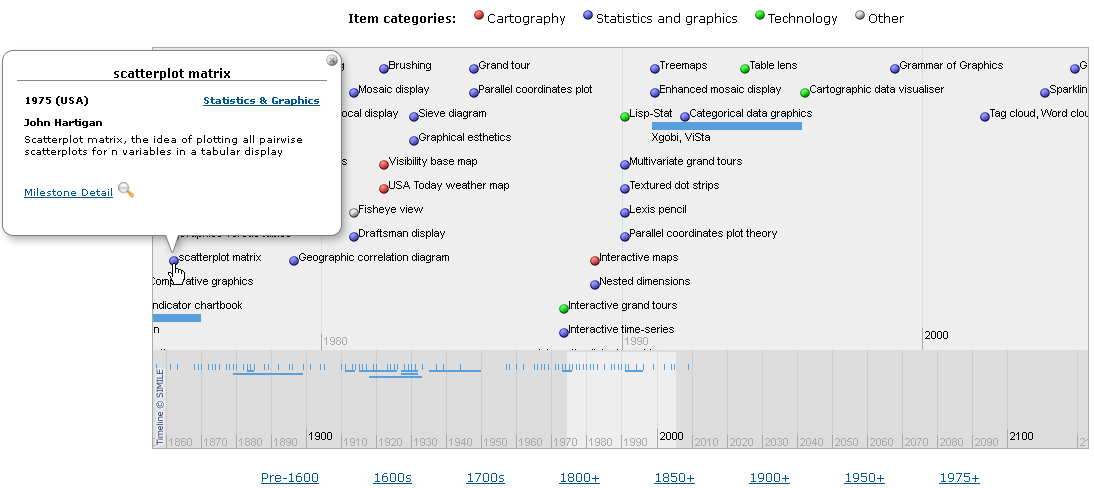
\includegraphics[width=\textwidth,clip]{fig/datavis-timeline2}
  \caption{Timeline view of the Milestones Project on the site \texttt{http://datavis.ca}. In this view,
  the top panel shows a detailed view of the segment of history highlighted in the bottom panel, both
  of which can be separately scrolled. Items in the top panel show a brief tag, color-coded in coarse
  categories. Clicking on an item in this panel brings up small description, linked to the details of
  the milestone item.
  }
  \label{fig:datavis-timeline2}
\end{figure}

It soon became apparent that such a text-based representation was inadequate. Updating the milestones data 
required that the single \LaTeX\ file be shared between multiple collaborators over email, and milestones 
assets, such as images or URLs were stored on a single computer not easily accessible by other collaborators.
As a result, collaboration with more than a few collaborators was cumbersome. The single file needed to be vetted 
at each iteration, and once enough data had been collected, rendered into a web site and manually uploaded so
that non-collaborators, namely the public, would be able to view the data.

Around 2005, we began to convert the flat file into a relational data and completely redesign the Milestones 
web site. Specifically, we wanted to facilitate collaboration between any number of collaborators via an easy
to use web administration area and allow for the dissemination of milestones data via an easy to browse public 
user interface, both of which would be tied to a relational database.

Migrating the data to this form provided some challenges. First, the existing milestones data needed to be
normalized and redundancy minimized. To do this, we broke the data into its relavent entities namely the 
milestone itself and its descriptors (aspect, author, subject, keywords, reference, and mediaitem).
The aspect, author, subject, keyword and reference descriptors exist as a many-to-many relationship between 
it and the milestone. For example an aspect can belong to one or more milestones and the mileston can belong to 
one or more aspects. While media items on the other hand, can belong to only one milestone at a time, with
multiple mediaitems possible for a single milestone. \figref{fig:datavis-schems-2} describes these relationships.

Normalizing the data in this way enabled us to free the databse of modification anomalies; ensured that database 
structure was scalable and could be extended with minimum mofications; made the relational model more informative 
to users; and made sure the data itself was query-neutral (Codd, 1971).

The second challenge related to how to display such a vast amount of information in an easy to understand
user interface...



\begin{figure}[!htb]
  \centering
  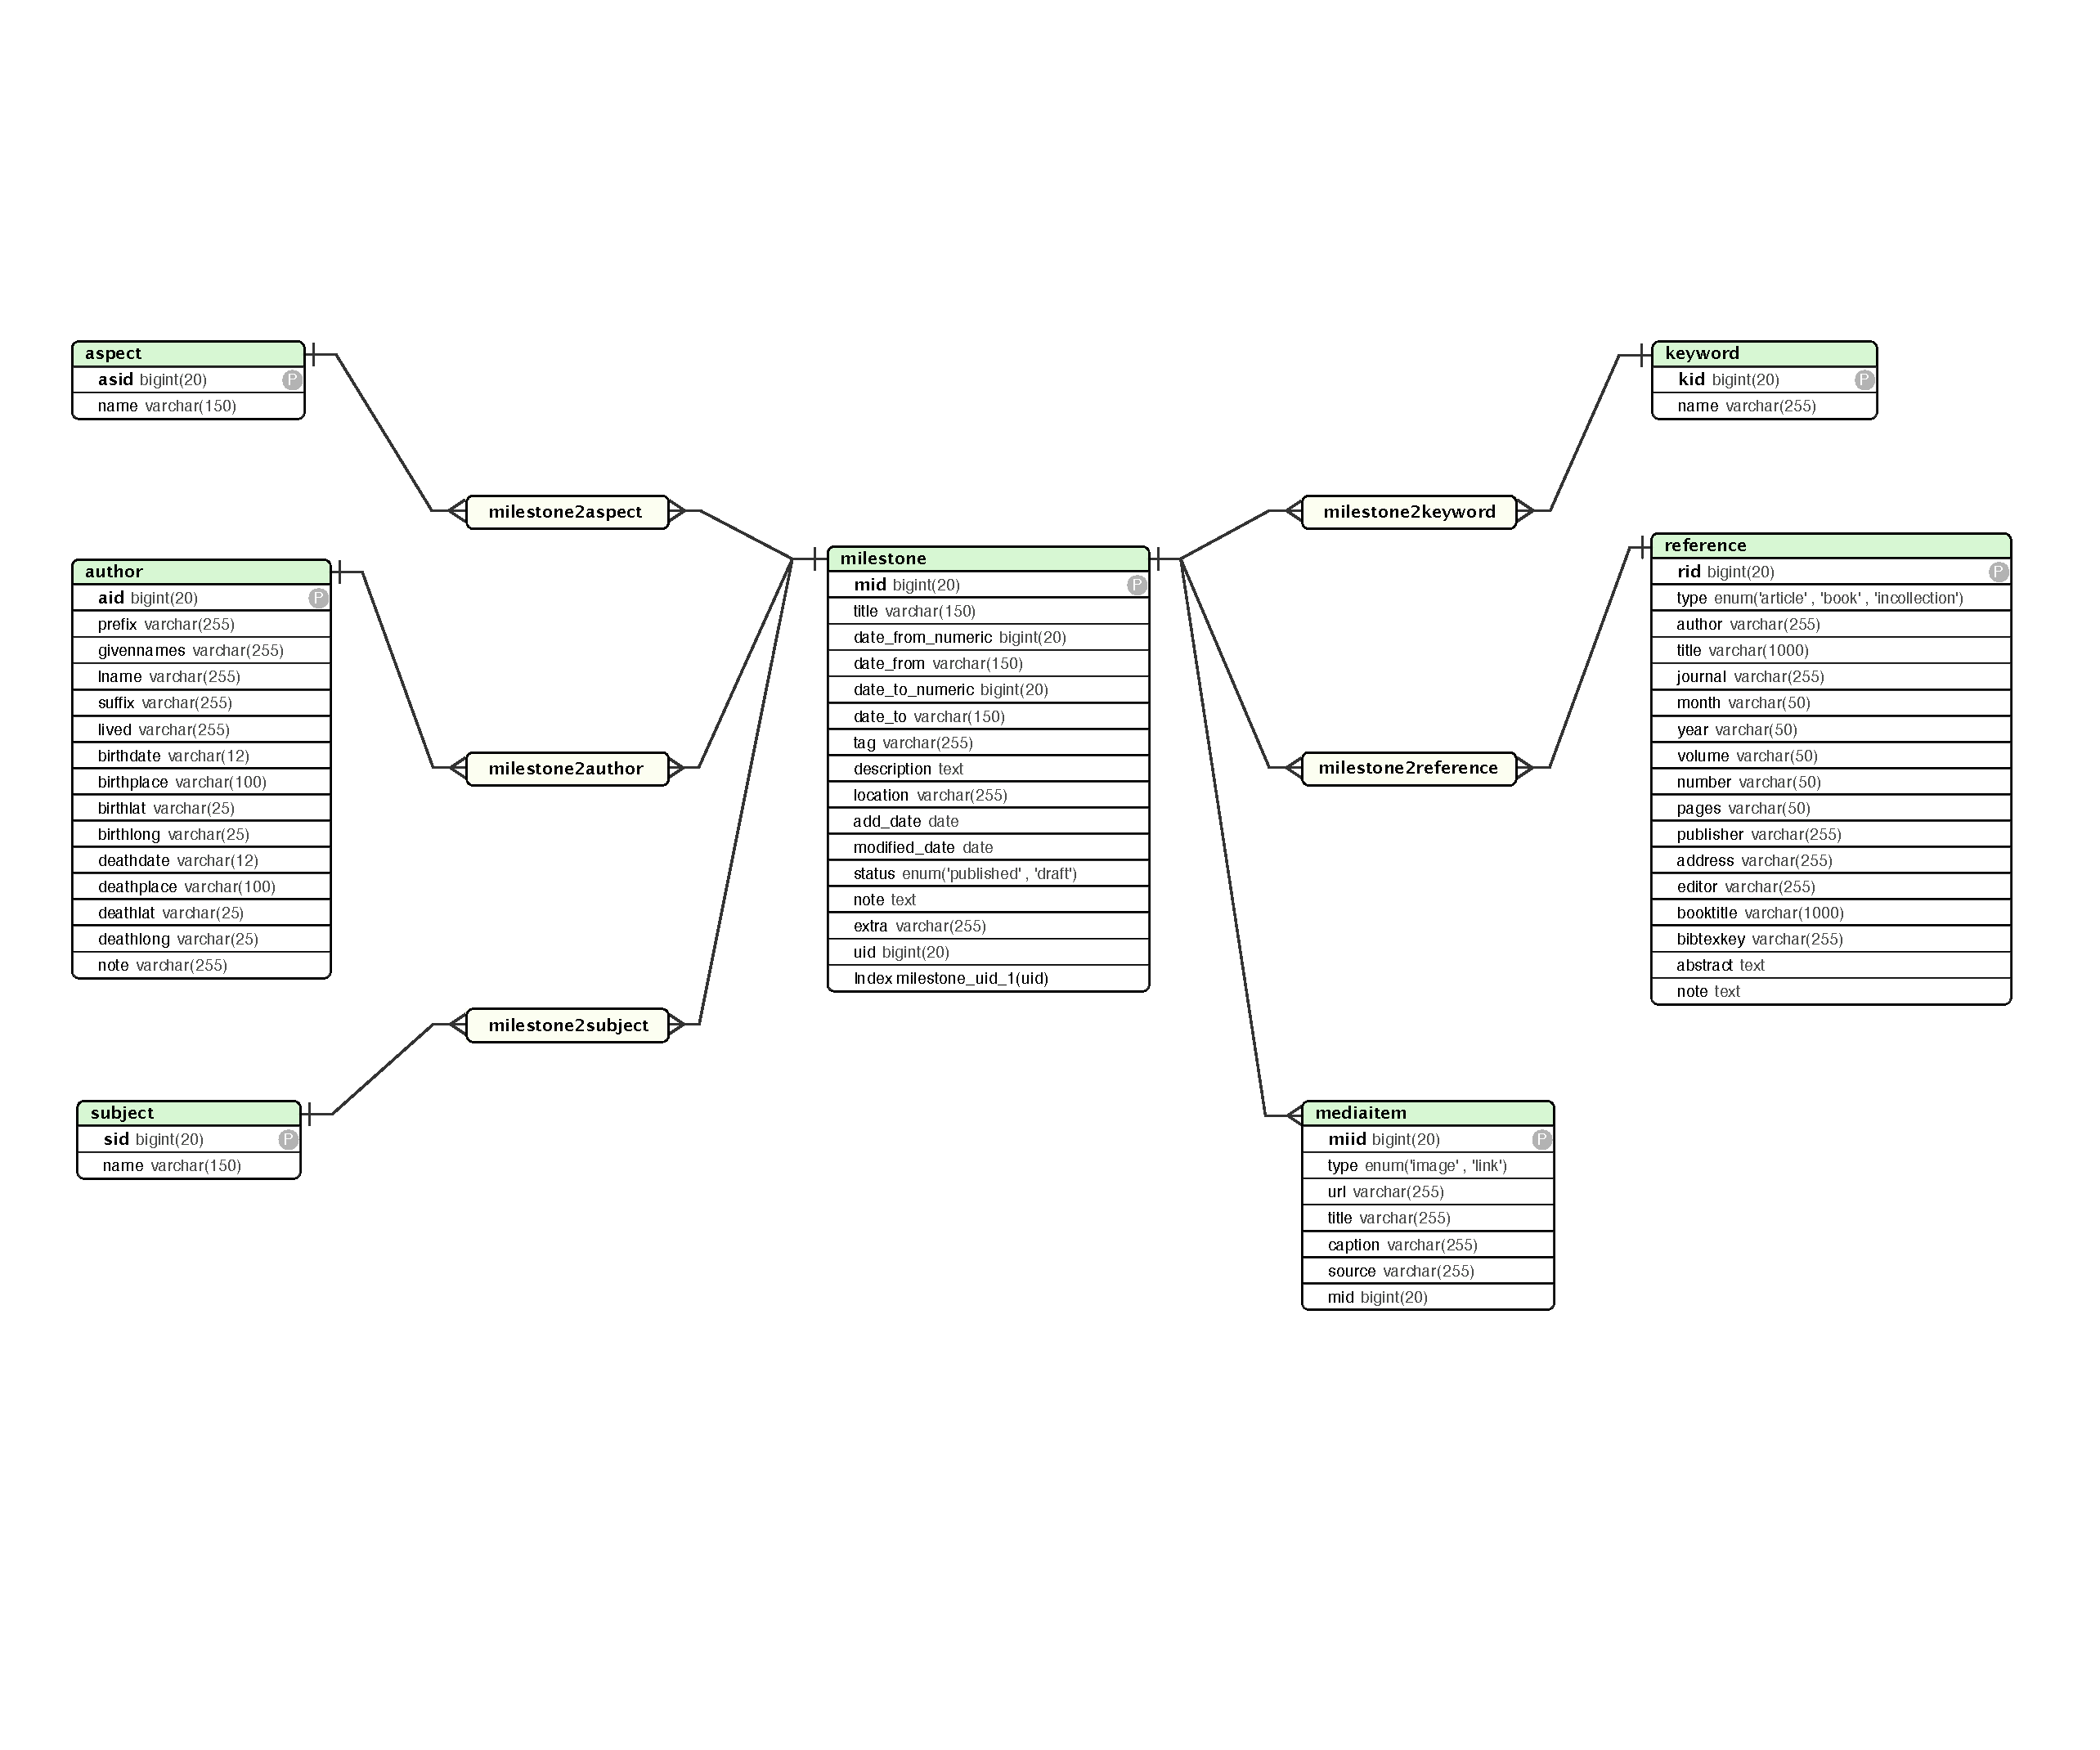
\includegraphics[width=\textwidth,clip]{fig/datavis-schema-2}
  \caption{Simplified schema for the MySQL database for the Milestones Project. The main 
  table (\texttt{milestone}) contains information regarding each of the items considered
  a milestone in the history of data visualization, linked to other tables 
  (e.g., \texttt{reference}, \texttt{mediaitem}) by unique (primary) keys.
  Other supporting tables (e.g., \texttt{milestone2aspect}) provide for convenient lookups of 
  descriptors of these milestones items (\texttt{subject}, \texttt{aspect}, \texttt{keyword}).
  }
  \label{fig:datavis-schema-2}
\end{figure}


At present, the Milestones Project lists 288 contributions to this history, with nearly 350 references,
information on 336 authors and 774 ``media items'', comprising 371 images appearing online on the
\url{http://datavis.ca} site and 403 links to images and documents at other sites.
In addition, we maintain an offline image database comprising over 1100 images collected from
various sources, ...

\figref{fig:datavis-timeline2} shows the timeline view of the miletsones items displayed on the
landing page. 

  % \S2
\section{Visualizing Time and History}\label{sec:vistime}
\begin{comment}
\begin{itemize*}
  \item Visions of history from the past
  \item Correlated pasts
  \item Non-linear scales
  \item Dynamic/interactive timelines
\end{itemize*}
\end{comment}
\epigraph{What does history look like?  How do you draw time?}{\citet[p. 10]{RosenbergGrafton:2010}}
The questions in this quotation from \emph{Cartographies of Time: A History of the Timeline} \citep{RosenbergGrafton:2010}
introduce an important topic in the history of data visualization: how to visualize this history?
Time provides one obvious dimension, but what else can be included to show the details of a history in a static display
or allow users to see more using dynamic and interactive displays?%
\footnote{Another recent book, \emph{Visualizing Time}
\citet{Wills:2012}, discusses a wide variety of modern graphical methods for visualizing time-based data.
} 

We have also provided an annotated visual gallery of some timeline designs and visual histories
in our Data Visualization Gallery at \url{datavis.ca/gallery/timelines.php}. The topics covered
include early visual histories, encyclopedic charts, special purpose charts, correlated histories
showing events in one domain in the context of events in other areas, non-linear scales for
time and space as well as dynamic, interactive timelines.  Here we just consider a few fresh examples.

\subsection{The first timelines, reconsidered}
Although there are earlier precursors, the first timelines of modern design---
a horizontal, linear axis for time and vertical positions for place, theme or category of events---
were produced in the mid 1700s, most notably Jacques Barbeau-Doubourg's 1753
\emph{Carte chronologique} and Joseph Priestley's 1765 \emph{Chart of Biography}.

Priestley first published a small ``Specimen'' of this chart as a proof-of-concept,
showing the lifespan of famous men in the years 600 BC to 0 AD, classified as
``statesmen'' (Solon,  $\dots$, Julius Caesar) and ``men of learning'' (Pythagoras, $\dots$, Ovid).
In the same year he published the detailed version \citep{Priestley:1765}
 that quickly became the most popular
and influential timeline of the \Cent{19} and for many years to come.  It showed the
lifespans of more than 2000 people from 1200 BC to 1750 AD, classified by their areas
of achievement (statesmen \& warriors, mathematicians \& physicians, artists \& poets, $\dots$).

\begin{figure}[!htb]
  \centering
  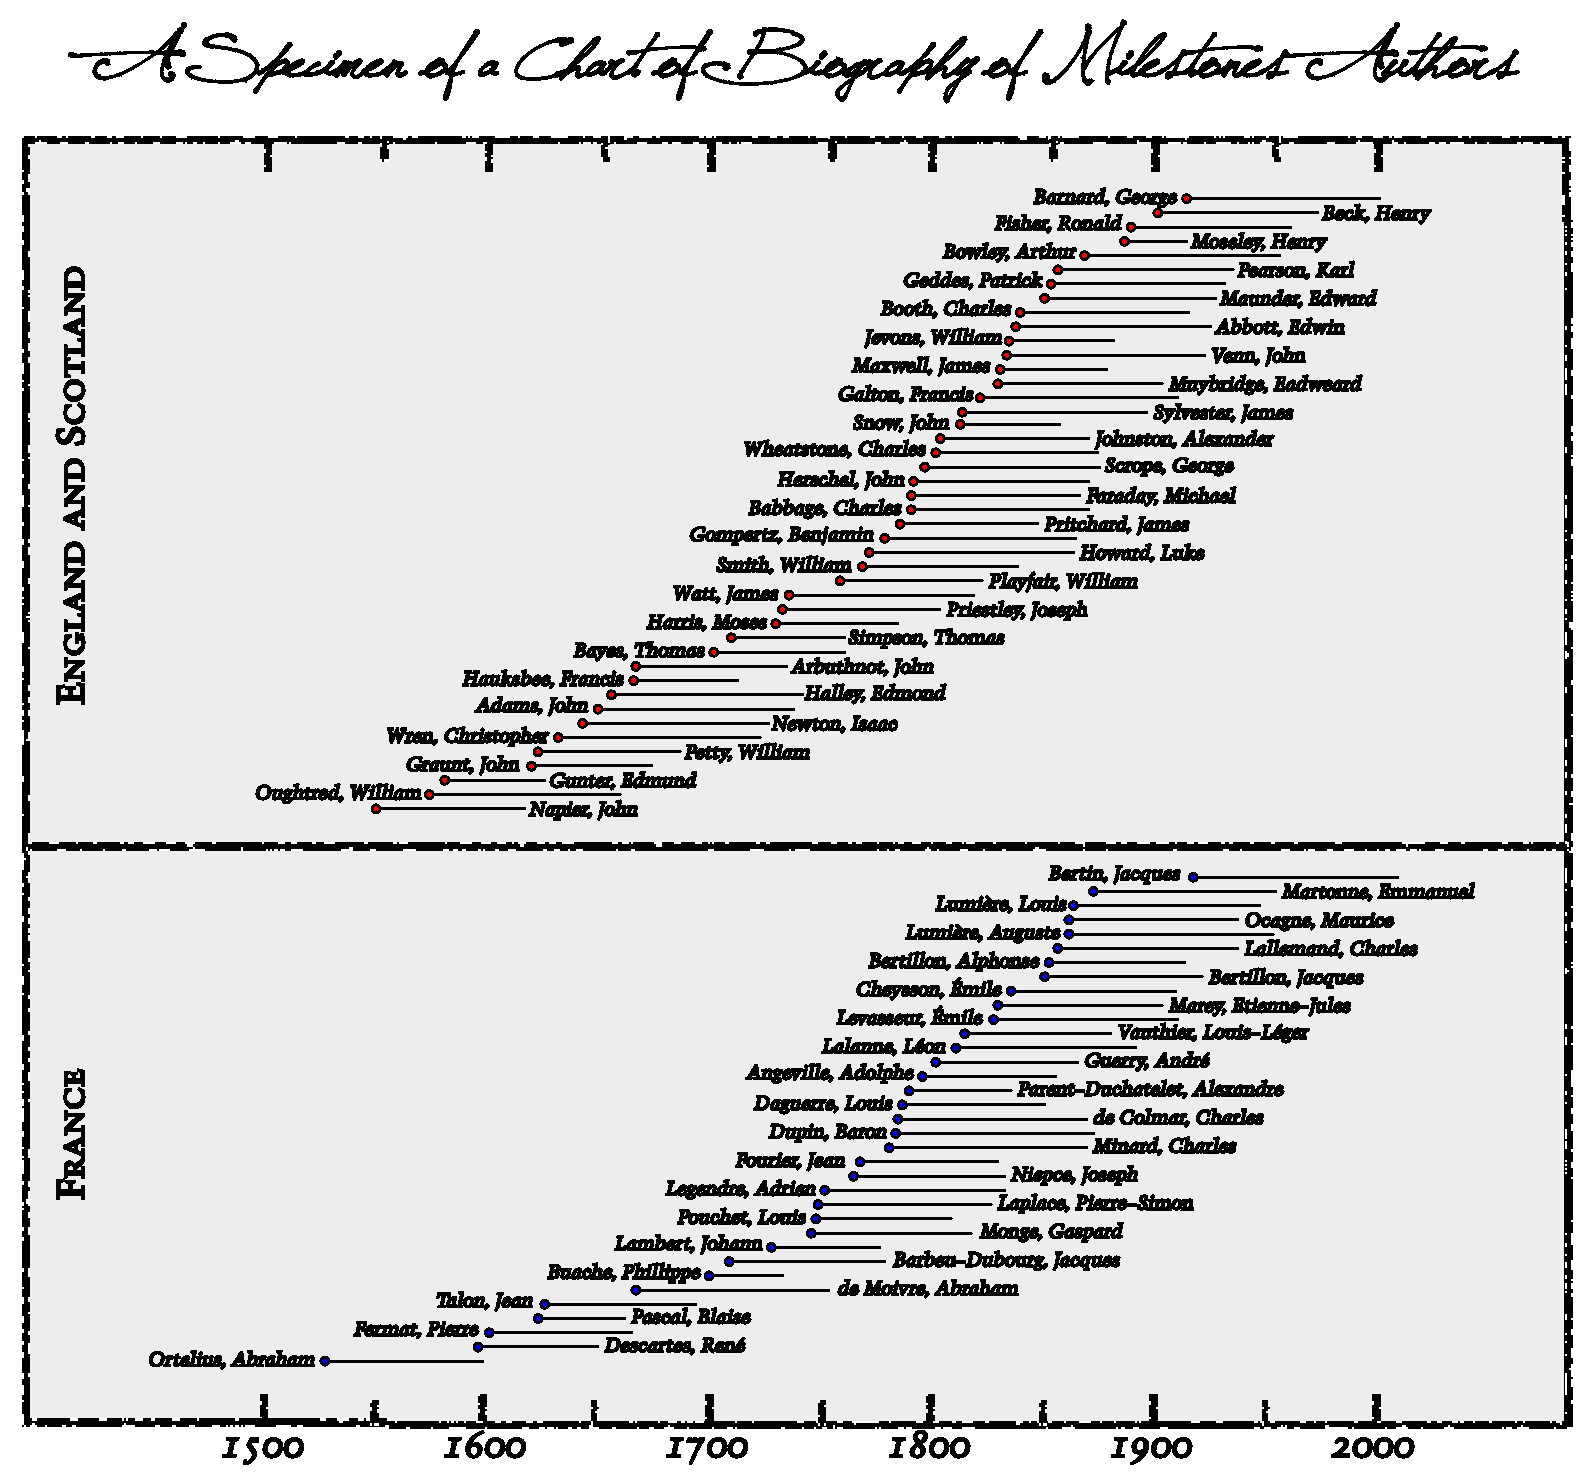
\includegraphics[width=.85\textwidth,clip]{fig/timespan}
  \caption{A modern re-design of Priestley's 1765 \emph{Chart of Biography},
  using information on authors in the Milestones database born in France or the
  United Kindgom. Authors are sorted within country by year of birth and labeled
  alternately at birth and death years, allowing both better lookup and visual
  comparison.
  }
  \label{fig:timespan}
\end{figure}

Priestly's timeline charts can be seen on our Data Visualization Gallery, and we don't reproduce
them here.  Instead we show (\figref{fig:timespan}) a re-design, in his style, of the lifespans
of 79 authors from the Milestones database who were born in France or the United Kindgom between
1500 and 2000. 

\citet[p. 117]{RosenbergGrafton:2010} call Priestley's charts ``masterpieces of visual economy.''
Indeed, they were at the time.  However, in his charts, the famous people were arranged 
haphazardly within category groups, so it is difficult to find specific individuals, 
and nearly impossible to see any trends, over time, or across categories. 

In our version, authors are sorted by birth year within each country and the names are printed
alternately at the year of birth and death. The result, which resembles a cumulative distribution
plot: (a) allows easier visual lookup of names, (b) provides an overall ``lifespan envelope,''
and (c) highlights a few individuals who lived conspicously shorter or longer than their
contemporaries (e.g. shorter: Willam Jevons,  James Maxwell, John Snow, Phillipe Buache).

Of course, to display lifespan \emph{directly} requires a different kind of plot, but one that
would not have been even thinkable by Priestley in 1765.  We return to this question in
\secref{sec:lifespan} (see \figref{fig:lifespan}).


\subsection{Universal histories}
In addition to unrivaled thematic maps and statistical diagrams, the Golden Age of graphics also
gave rise to a variety of novel attempts to visualize history in a comprehensive manner,
combining parallel, intertwined time-flows, text, illustrations, maps and other visual forms.
Among the most impressive is a series of Synchronological Charts of Universal History
produced by Sebastian Adams between 1871--1885.
The 1881 version is 23 feet long and shows 5,885 years of history, from 4004 B.C. to 1881 A.D.
\citet[p. 172]{RosenbergGrafton:2010} call it ``nineteenth-century America's surpassing achievement in complexity and synthetic power.'' 

\figref{fig:Adams1881} shows just a small portion, but the entire chart can be viewed at
\url{http://www.davidrumsey.com/blog/2012/3/28/timeline-maps}.  Adams used a linear scale for
time, and so you can understand why it took 23 linear feet to include all of recorded history.

\begin{figure}[!htb]
  \centering
  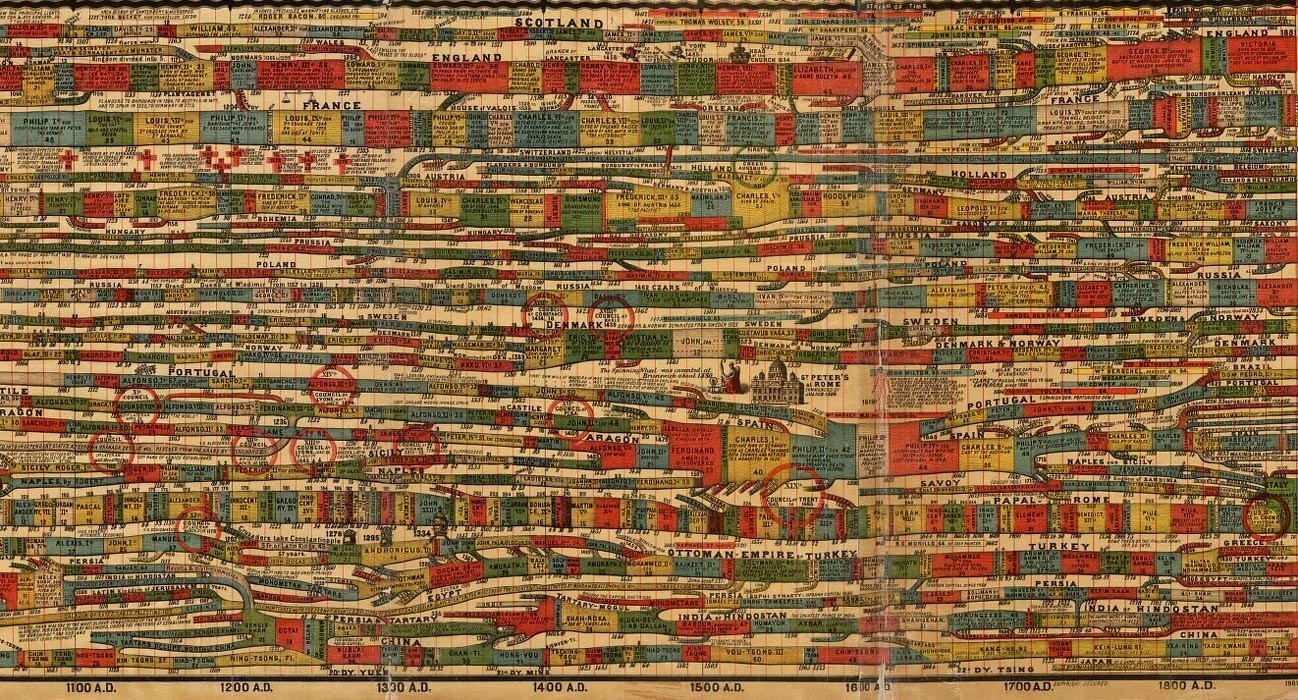
\includegraphics[width=\textwidth,clip]{fig/Adams1881-4}
  \caption{A portion of Sebastian Adams' \emph{Synchronological Chart of Universal History}, 1881,
  covering the \Cent{11}--\Cent{19}.
  The horizontal bands trace developments in different countries, with detailed text describing significant
  events, and which break up or merge according to political factors.
  }
  \label{fig:Adams1881}
\end{figure}

\subsection{Categorization and non-linear scales}

Linear time scales have the advantage that they
provide uniform resolution and detail across the entire time span, but events in time, or our interest in them are rarely uniformly distributed. Most visual histories are rather sparse at their beginning and very
crowded at their end.
Non-linear scales allow resolution to vary smoothly in some other way, providing for greater detail
in regions of greater interest, most often the recent past.


\begin{figure}[!htb]
  \centering
  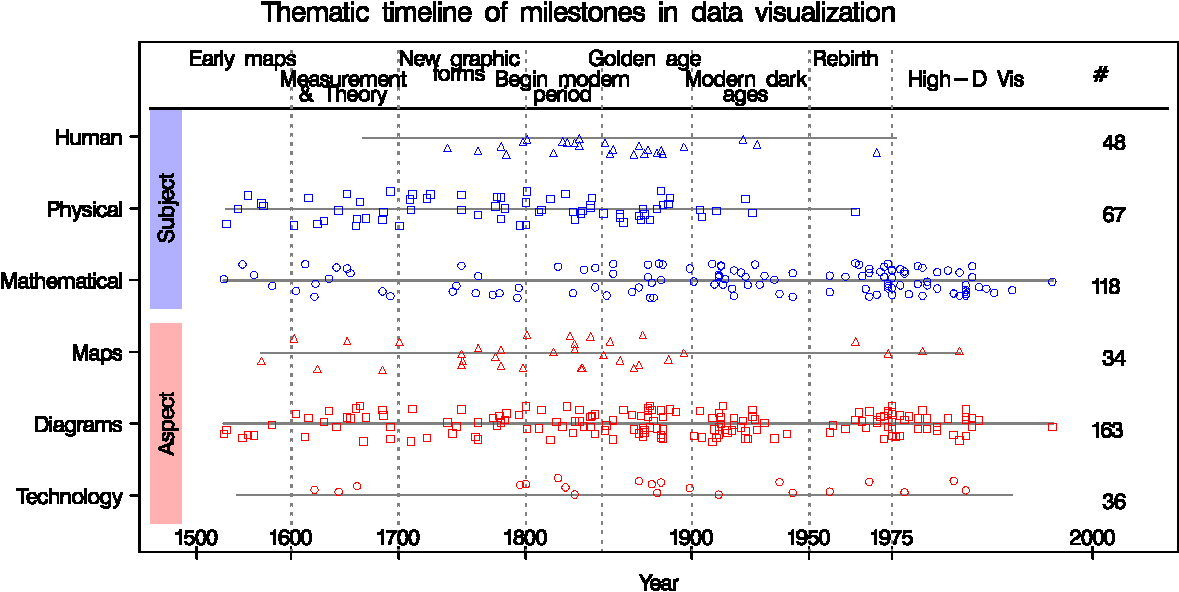
\includegraphics[width=\textwidth,clip]{fig/milecatline}
  \caption{Sketch for a thematic timeline of milestones items, 1500--present,
  categorized by both the Subject (content)
  and Aspect (form) of the milestone item.  To provide greater resolution for more recent events,
  time (Year) is shown on a square-root scale, going backward from the year 2000.
  }
  \label{fig:milecatline}
\end{figure}

\figref{fig:milecatline} is really just a proof-of-concept sketch for something that a graphic artist
could use as a starting point for a chart of
the history of data visualization. It uses the events from the
Milestones Project, categorized by two correlated factors: 
Subject area or content has been
categorized as dealing with human populations, physical properties of the world or
mathematics and statistics; aspect or form has been categorized as dealing with
cartography, graphs and diagrams or technology 

To provide greater resolution for more recent events, we have used a reverse square-root
scale going backward from the year 2000. Specifically, Year on the horizontal time axis
is actually plotted according to the formula $\textrm{Year}^\star = 2* (25 - \sqrt{(2000 - \textrm{Year})})$,
giving the more pleasing result that the modern period 1800--2000 occupies about 60\% of the scale,
although it comprises only 40\% of the range.

  % \S3
\section{Using the Milestones Project for Statistical Historiography}\label{sec:historiography}
\epigraph{Vision is the art of seeing things invisible.}{Johnathan Swift, 1711}

\begin{comment}
\begin{itemize*}
  \item comparisons of graphical innovations by field (e.g. physical sciences vs. social sciences), in terms of content and form
  \item extract themes and relationships between content areas
\end{itemize*}
\end{comment}

\subsection{Statistical historiography}\label{sec:stathist}
We use the term ``statistical historiography,'' to refer to the use of statistical and graphical methods to explore, study and describe historical problems and questions.%
\footnote{As far as we know, the initial expression of this idea appeared in a paper by \citet{Rubin:1943} discussing various ways in which statistical methods could be applied to historical topics.  These included: the use of sampling methods to test historical theories; statistical distributions applied to historical data; and, the use of time series graphs with smoothed curves to study historical trends. More recently, many examples of the application of these ideas to statistical topics can be found in \citet{Stigler:1986,Stigler:1999}, as well as our own papers on the history of data visualization, cited \emph{inter alia}.}
This topic has a delightful self-referential quality when applied to the history of data visualization itself, since we have often found ourselves using modern methods of statistical analysis and graphics to study the development of ideas in this area. As in the quotation from Swift above, one goal is to make previously hidden aspects of this history visible.

At the same time, our examination of some of the most impressive graphic works of the past sometimes left us awe-struck by their exquisite beauty and visual design.%
\footnote{Some examples are: Charles Joseph Minard's famous depiction of Napoleon's March on Moscow \citep{Friendly:02:Minard}, Francis Galton's detailed study of weather patterns in Europe \citep[see:][]{Friendly:2008:golden}, and Andr{\'e}-Michel Guerry's \citep[Plate 17]{Guerry:1864} semi-graphic table depicting the relations of occurrence of crimes to a wide variety of social and demographic factors \citep[see:][]{Friendly:2007:guerry}.}
On more than one occasion when looking at these elegant presentations, we wondered whether there wasn't something lost with the advent of modern software. While we can now analyze massive data sets, and generate a multitude of graphics with a simple mouse click, we still feel that designing a truly effective visual display of information requires thought and manual intervention.

For this reason, it is often quite instructive to attempt to re-create or even re-vision a graphic work from the past \citep{Friendly:02:Minard}. 
We can learn from this undertaking an appreciation for the insight and hard labor of our graphic heros, and can sometimes better understand 
or improve on their designs by a process we call ``understanding through reproduction,'' another facet of statistical historiography.

We illustrate this approach with an analysis of a graph from \citet{Playfair:1821}
shown in \figref{fig:playfair-wheat1}, in some ways a tour-de-force of
early graphic presentation. In this graph, Playfair used three parallel time
series in different forms
to show the price of wheat (bar chart), weekly wages (line graph), and reigning monarch (bars at the top)
over a $\sim$250 year span from 1565 to 1820. His graphic goal was rhetorical: he wished to
argue that workers had become better off in the most recent years. Surely this must be counted
among the best early data graphics.

%% one figure
\begin{figure}[htb]
  \centering
  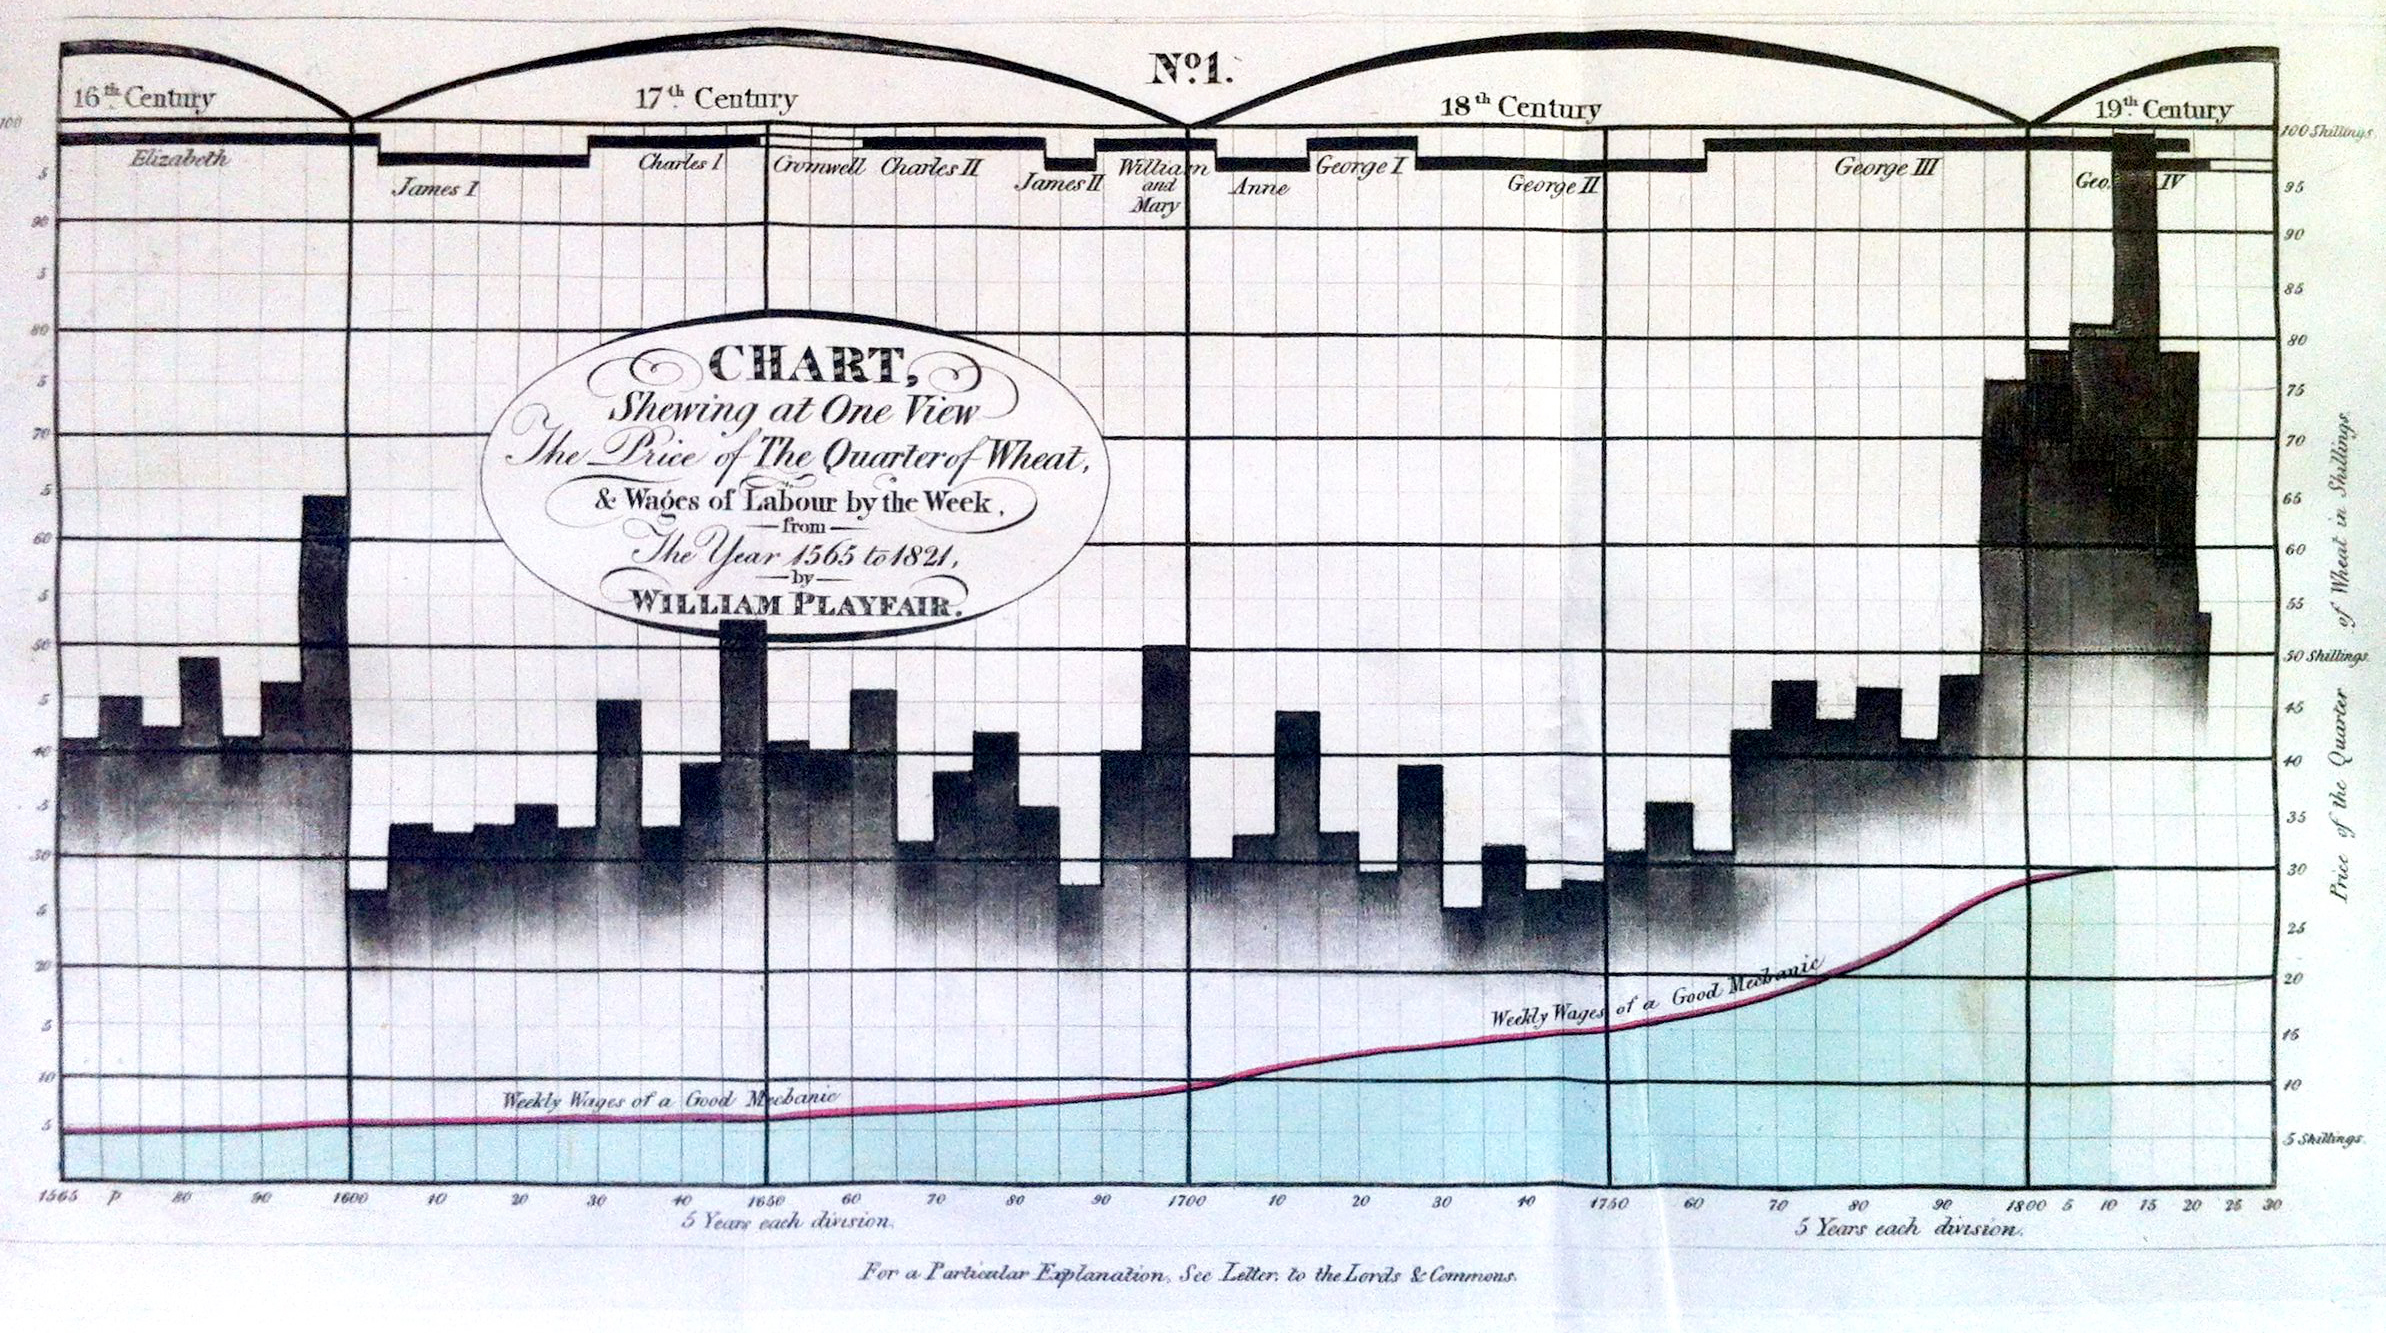
\includegraphics[width=\textwidth]{fig/Playfair1821b}
  \caption{William Playfair's 1821 time series graph of prices, wages, and ruling monarch
  over a 250 year period.
  \emph{Source}: \cite{Playfair:1821}, image from Stephen Stigler.}%
  \label{fig:playfair-wheat1}
\end{figure}

Yet, as we have argued elsewhere \citep{FriendlyDenis:05:scat}, this graph is both sinful
and a communication failure for Playfair's purpose.  It is sinful because the use of separate $y$ axes for
wages (left axis, range: 0--100) and prices (right axis, range: 0--30) on different scales
provides the opportunity to tell very different stories simply by re-scaling one or both
axes.

%% one figure
\begin{figure}[!htb]
  \centering
  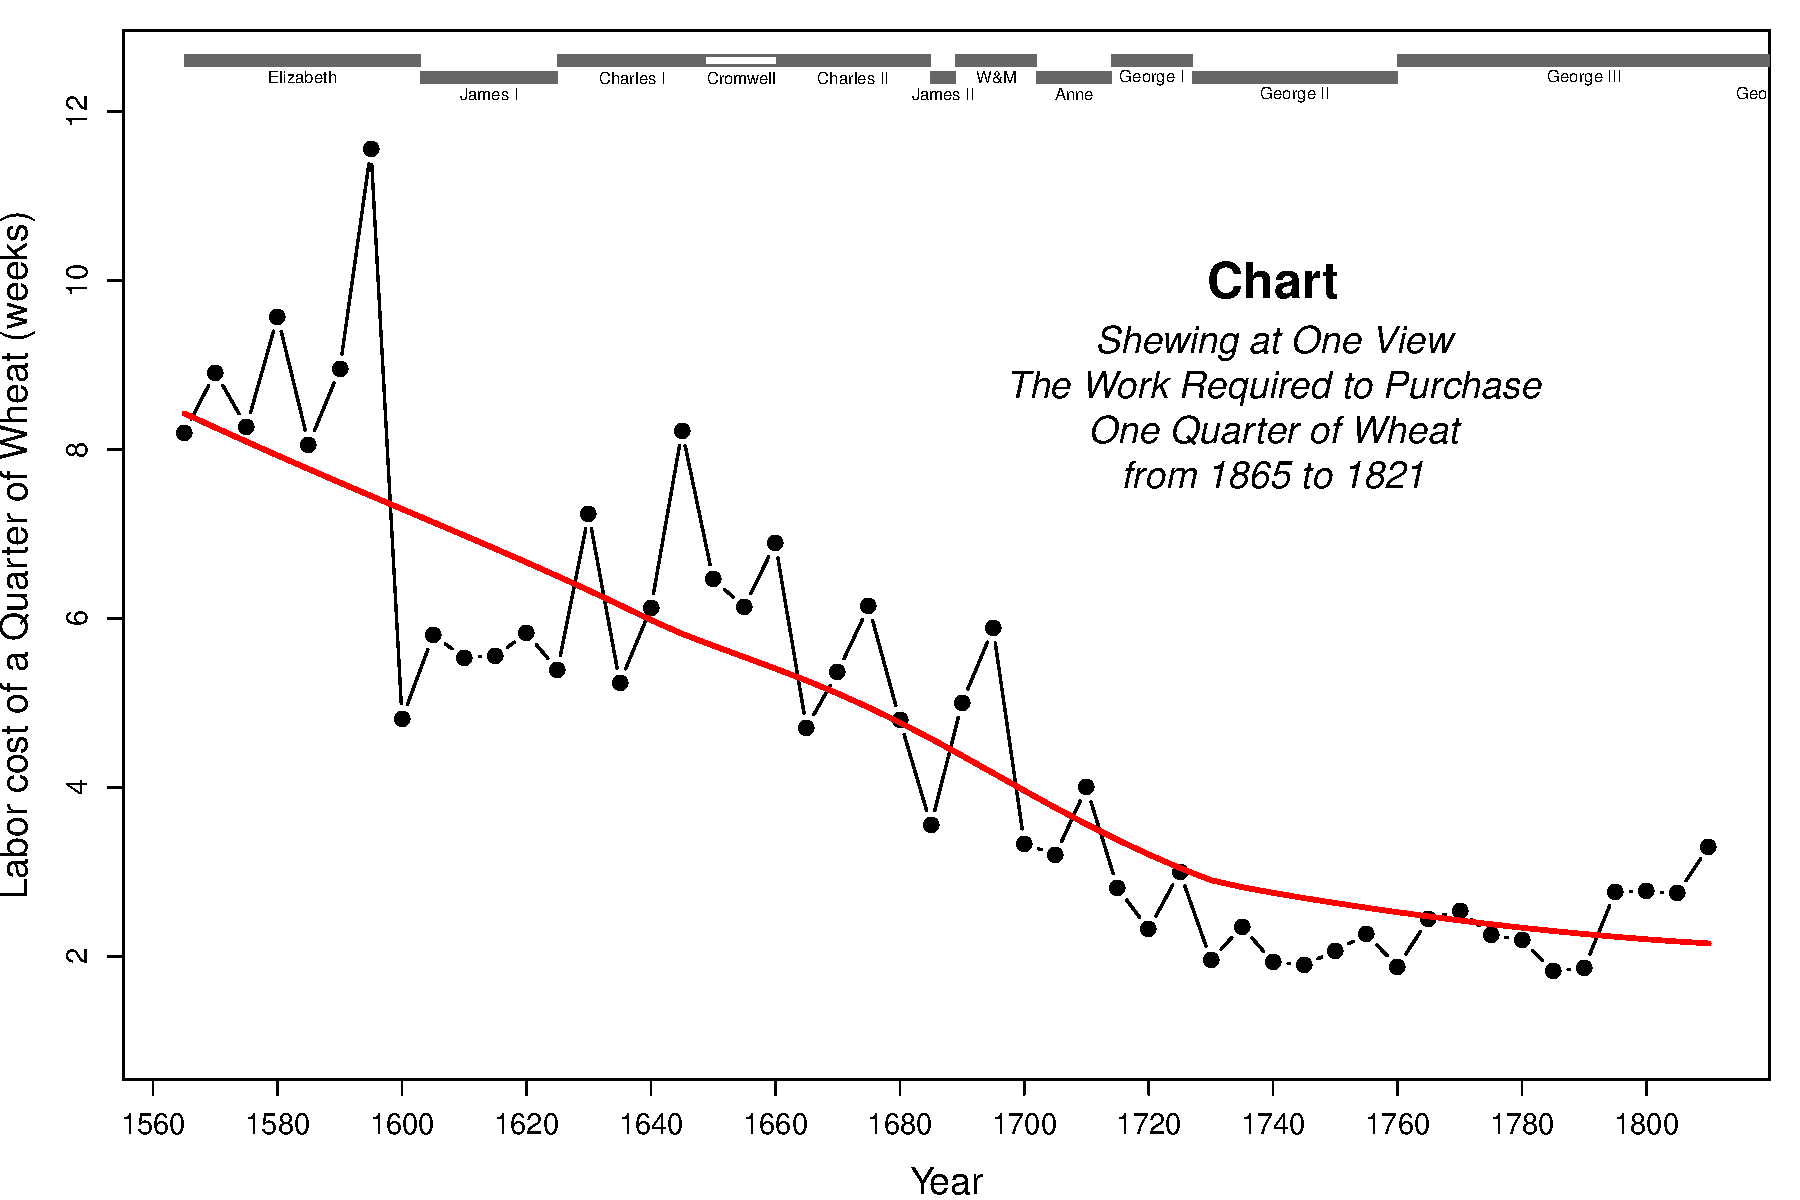
\includegraphics[width=.9\textwidth,clip]{fig/wheat2}
  \caption{Redrawn version of Playfair's time series graph
  showing the ratio of price of wheat to wages,
  together with a loess smoothed curve.}
  \label{fig:wheat1}
\end{figure}

It is also a graphic failure because the visual impression that wages increased relative to prices
toward the right end is at best indirect and is obscured by the large fluctuations in prices of wheat.
What Playfair might have done to show the relation directly, is to plot the \emph{ratio} of price to wages,
representing the labor cost of a unit of wheat, as we have done in \figref{fig:wheat1}.%
\footnote{
Playfair's data and this re-creation can be found in the \texttt{R} package HistData \citep{HistData}
as \texttt{example(Wheat)}.
}
Adding a non-parametric (loess) smoothed curve to the line plot makes Playfair's message directly apparent;
it also shows that the reduction in the amount of labor required to purchase one unit of week in fact
levels off in the last 40 years. As well, it highlights that something quite unusual happened around 1600.


However, in order to conduct such statistical historiography, there is one principal requirement: \textbf{data}. The Milestones Project database is the repository of all the information we have so far recorded, and modern database tools allow the possibility of simple or complex queries, limited only by the available information.%
\footnote{It should be noted that, beyond the basics of recording milestones items, images and references, inputting the other meta-data (content and form categories, keywords, etc.) is highly labor-intensive. Thanks are due to many research assistants and graduate students who have and continue to work on the Milestones Project, including Dan Denis, Matt Dubins, Yvonne Lai, Avi Lipton, and Carolina Patryluk.}
In related work, we have collected and disseminated data sets of historical interest on a variety of topics in statistics and data visualization, for instance via the \texttt{R} packages HistData \citep{HistData} and Guerry \citep{Guerry}. These can be considered another source for data, pictures, and stories related to statistical historiography, and understanding through reproduction. This is the essence of the motto on the \url{datavis.ca} web site: \emph{Looking back, going forward}.

In the subsections below, we describe a few applications of these ideas using the Milestones Project database and case studies that arose from this work. There is an interesting interplay between such historical analyses and these data collections. Some studies called for us to find and incorporate new data sources, such as our paper \citep{Friendly:2007:guerry} on Guerry's \emph{Moral statistics of France} and the Guerry package, to which we added Angeville's extensive 1836 data on social and economic characteristics of France. In other cases, our analyses suggested new or different ways to visualize historical data.

\subsection{Milestone authors: lifespan}\label{sec:lifespan}
As noted earlier, we record information relevant to the contributors of milestones events in an author table in the database. For most of these individuals, internet and biographical searches allowed us to determine the dates and places of their birth and death.

One simple question that can be posed using this information is how long did these contributors live? As illustrated earlier (see \figref{fig:timespan}), Joseph Priestley was the first to develop the idea of using a graphic representation to show the lifespan of famous men. His ``charts of biography'' did this in a particularly evocative form, representing each person by a line segment whose length was defined by the individual's lifespan, and then grouped by occupational category.

These ``timespan'' charts tell an interesting story, but they do not provide an answer to the question of how long, in general, these individuals lived.  However, with the author table from the Milestones Project, it is a simple matter to calculate lifespan, and obtain a direct answer to this query. \figref{fig:lifespan} shows one display of this information, using a combined density plot and rug plot, similar to the one used in \figref{fig:mileyears4}.

\begin{figure}[!htb]
  \centering
  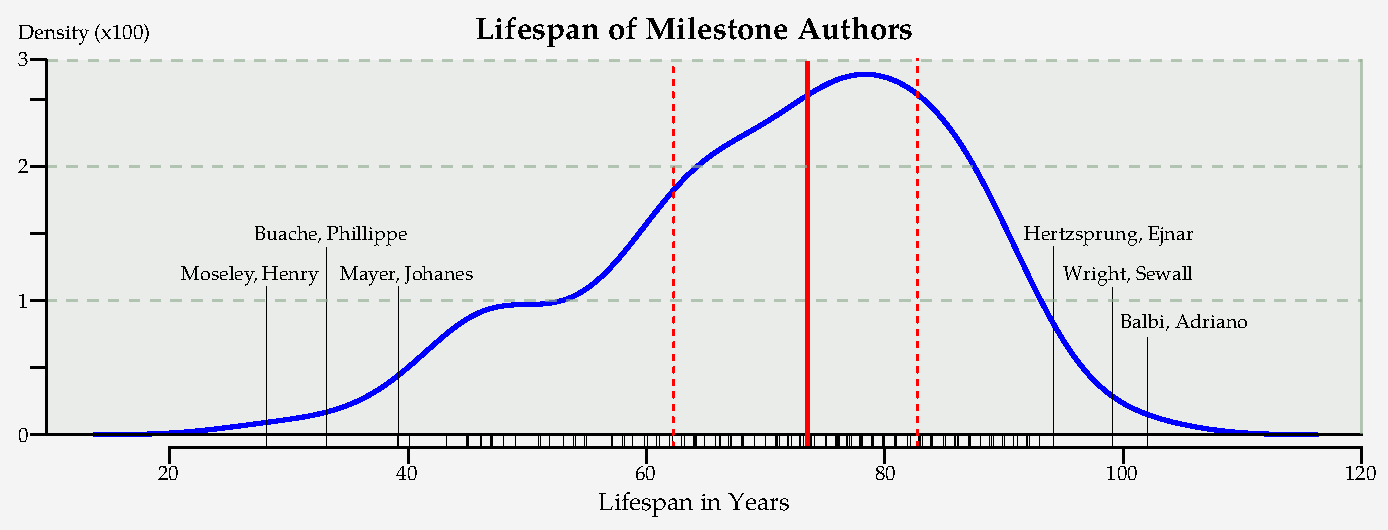
\includegraphics[width=\textwidth,clip]{fig/lifespan3}
  \caption{Density plot of the lifespan of the 172 authors in the Milestones Project database who were born after 1500 and for whom lifespan can be determined. Individual observations are shown by a (jittered) rug plot, and the three extremes on each end are identified by name.  The red vertical lines show the quartiles of the distribution.}
  \label{fig:lifespan}
\end{figure}

Several features of this plot deserve comment, and also invite further inquiry: Most notable is that, by and large, milestones authors generally lived to a ripe old age--- the median lifespan is 73.0, but the density plot peaks at around 79. This contrasts with a detailed study on famous people between 2400 BC to 1880 AD by David de la Croix and Omar Licandro (\url{http://www.fcs.edu.uy/archivos/BCU_clebrities.pdf}).  In their research, it was found that the typical lifespan fluctuated around a mean of 61 years for four millennia, and only gradually reached 69 toward the end of their sample. Such a discrepancy between the two studies might warrant further investigation; for instance, by classifying the individuals into occupational, locational, or otherwise more delineated groups, and looking for trends.

Another interesting feature that becomes apparent in this graphic is the noticeable bump in the distribution around 45 years. This occurrence calls for some attempt at further explanation. We don't pursue this here, but again note that such graphs often suggest further analyses (breakdowns by region or time period), or cry out for the collection of more data.

Finally, although \figref{fig:lifespan} is just a summary graph, we have labeled a few extreme observations on each end, which may relate to telling parts of the story of the history of data visualization.  Among these, Henry Moselely, who is known for the discovery of atomic number from a graphical display, died the youngest, as a consequence of serving in the British Army during World War I. But, we were surprised to see the noted and prolific French cartographer Phillippe Buache, and the German physicist and astronomer Johann Tobias Mayer, show up in positions two and three.  On the other end, we were delighted to see that Adriano Balbi, a Venetian geographer and early collaborator of Andr{\'e}-Michel Guerry \citep{BalbiGuerry:1829} had the longest lifespan, just exceeding the population geneticist, Sewall Wright, who invented path analysis and the path diagram around 1920.  By incorporating these details, the visualization is able to reveal narratives that otherwise would have been concealed.

\subsection{Milestone authors: geography}\label{sec:geography}
The Milestones Project web site provides an initial page showing an interactive timeline of the events in this history as a visual overview (\figref{fig:mileyears4}). A long-term goal has been to provide other views of this history and other tools for searching and exploring the database. With recent technological developments, it became evident to us that one such method would be through the use of geographical data.

So far, the primary geographic information we have encoded in the database refers to the birth and death place of the milestone authors. This is an imperfect representation, as these locations may not accurately represent the author's primary residence.  For instance, Charles Joseph Minard was born in Dijon, and died in Bordeaux, but all of his work was done in Paris while he worked at the {\'E}cole Nationale des Ponts et Chauss{\'e}es. Nevertheless, a geographic view of the available information is potentially useful. In this regard, we used the Google geocoding tools to provide latitude and longitude for the locations listed in the author table.  Using this and the R package googleVis \citep{googleVis}, we created the interactive map shown in \figref{fig:authormap}.

\begin{figure}[!htb]
  \centering
  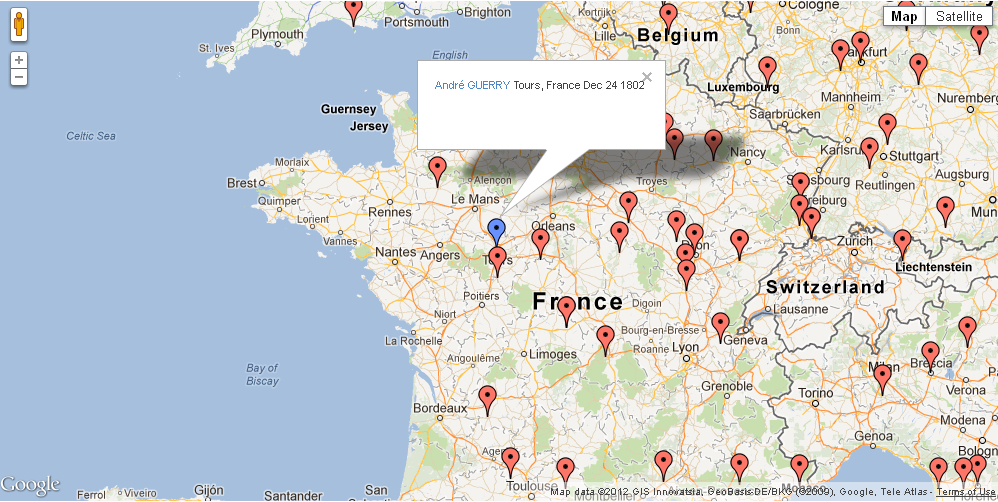
\includegraphics[width=\textwidth,clip]{fig/authormap}
  \caption{Birth places of 188 milestone authors, shown on an interactive Google map, centred on France. Each geographic marker is linked to an author query on the \texttt{datavis.ca} web site that lists the contributions by that individual.}
  \label{fig:authormap}
\end{figure}

Like other instances of Google Maps, this graphic can be panned and zoomed using mouse controls. The place markers display tool tips when hovered over and, when clicked, link to a search page that details all of the Milestone items that are related to that author. This interesting visualization will soon be revealed on the Milestones Project website, with future work planned to incorporate other types of data in addition to the birth and death locations.

\subsection{Milestones: themes and trends}\label{sec:themes}
The records in the Milestones Project database also feature various text fields for each logged event. These include a brief item tag, a full description of the event, and relevant keywords, as well as categorical codes for the content (Subject), and form  (Aspect) of the item. Treating this information as ``data'' allows us and others to study themes and trends in these developments.  Modern methods of text mining and data visualization can provide insights into this history not available through other means.

As one simple illustration of this approach, \figref{fig:milecats4} shows two mosaic displays%
\footnote{Mosaic displays show the frequencies in cells of a cross-classified table by the area of each tile.  The tiles are shaded according to departure from a null
model of no-association, using blue for cells with frequencies substantially greater than chance, and red for cells with frequencies that are lower than expected.}
that explore the relationships among Epoch, Subject, and Aspect. The left panel shows changes in the distributions of milestone events by Subject over time.  It can readily be seen that while most of the milestone innovations up to the end of the \Cent{18} were about the physical world (astronomy, geodetic measurement, weather, etc.), this trend changed in the \Cent{19}, where there was a large shift toward problems that related to human populations (e.g., pertaining to mortality, births, disease, crime). Beginning in the early 1900s, the pattern changes again, with advances in mathematics and statistics becoming the dominating force.

\begin{figure}[!htb]
  \centering
  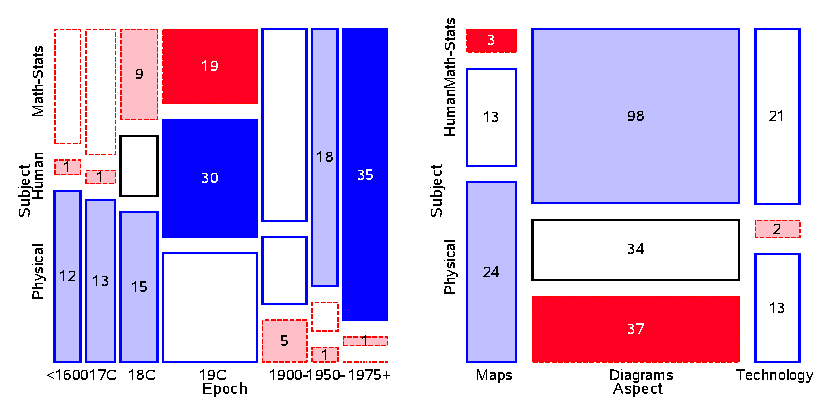
\includegraphics[width=\textwidth,clip]{fig/milecats4}
  \caption{Mosaic displays for milestone items, classified by Epoch, Subject and Aspect. Left: mosaic for the marginal table showing differences in Subject across Epochs; Right: mosaic for the marginal table showing differences in Subject across Aspect. Numbers in the tiles give the number of milestone items.}
  \label{fig:milecats4}
\end{figure}

The right panel shows the association between Subject and Aspect, pooled over Epoch. As is not surprising, maps and other cartographical representations were most often used to show data of the physical world, while graphs and diagrams were most often associated with mathematical and statistical subjects.

Other statistical graphs and analyses could be used to explore these and other relationships in more detail. The key to this is of course the existence and availability of data--- in this case reflected by the coding of graphical milestones in our database.
  % \S4

\section{Conclusion and Future Directions}
The Milestones Project began as a simple attempt to collect a comprehensive history of innovations and developments in data visualization in a single, ``one-stop shopping'' location. Like Topsy, it ``just grew'' over time, with images, historical papers and references, suggestions, and other contributions graciously provided by friends and collaborators, most notably from the members of \emph{Les Chevaliers des Albums de Statistique Graphique}.

In this chapter, our primary goal was to introduce the second and latest iteration of this project.  The redesign was undertaken to make this history more accessible for browsing and searching, and to attempt to make the database more amenable to additions, edits, and extensions among collaborators.  However, we find that the most exciting aspect of the new structure is its flexibility in terms of data retrieval, 
and our newfound ability to use and manipulate the data for graphic-based statistical historiography.

One goal for the future, as we suggested earlier (\secref{sec:geography}), is to extend the user interface to provide multiple
views and advanced text search and filtering capabilities.
One convenient path for this development is provided by the SIMILE Exhibit framework
(\url{www.simile-widgets.org/exhibit3/}).  This provides web software libraries (Ajax, javascript, css) for
timelines, interactive maps, tabular displays, image ``tiles'' and other visualizations.
Various views can be composed for browsing as tabbed, alternatives or as faceted displays, showing, for example an interactive timeline and
a map.

Equally important, the Exhibit framework allows us to present some of the milestones tables to be used as filters for the items
displayed in these views.  Tables for subject, aspect, keywords, location, epoch, etc. would allow the user to select
select milestone events based on some or all of these criteria, providing a way to ask such questions as
``what milestones events between 1700-1900 involving social science occurred in Europe?'' 

Finally, we would like to make the milestones database more publicly accessible for use by others on the history of data
visualization.  For the examples we have shown here, we connect to the milestones database directly via MySQL or ODBC
interfaces to SAS and R, but this presents security risks.  Happily, the Exhibit framework also provides methods for
data export from various views, using JSON or CSV formats. In addition, we contemplate adding facilities for users in
the data visualization community to add comments, notes, references and links to milestones items.
These extensions will comprise the Milestones Project 3.0.

%\bibliography{graphics,timeref,Rpackages}
\bibliography{FriendlySigal2012}        % after being processed bibtool -- quiet=on -r ~/texmf/bibtex/bib/aux2bib.rsc -x FriendlySigal2012.aux -o FriendlySigal2012.bib
\end{document} 